%\chapter{Discussion}
%~~~~~~In COMET experiment, the radiation will cause the damage of the superconducting maget which is possible to lead that the temperature rises up to the current sharing temperature.
%Here, we are going to discuss the margin of calcualtion and optimization of CS1 coils.
%
%\section{Margin of Monte Carlo code}
%~~~~~~As mentioned in previous chapter, different result of neutron production and energy deposition is obtained in terms of different physics model.
%Nowadays' heat calcualtion bases on the model of JAM\_INCL\_JENDL.
%We suppose there is fator of $\pm$0.3 in different physics model.
%The figure~\ref{5factor} shows the temperature changes with the factor of energy deposition for 90 day operation.
%The maximum temperature grows up with factor.
%Supposed that the energy deposition predicted by the other physics model is higher than JAM\_INCL\_JENDL by factor 1.5, cooling for 30 days is not allowed for phase-II experiment.
%Thus, the energy depostion and neutron production is necessary to be checked correctly by using different physics model in future.
%\begin{figure}[H]
% \centering
% 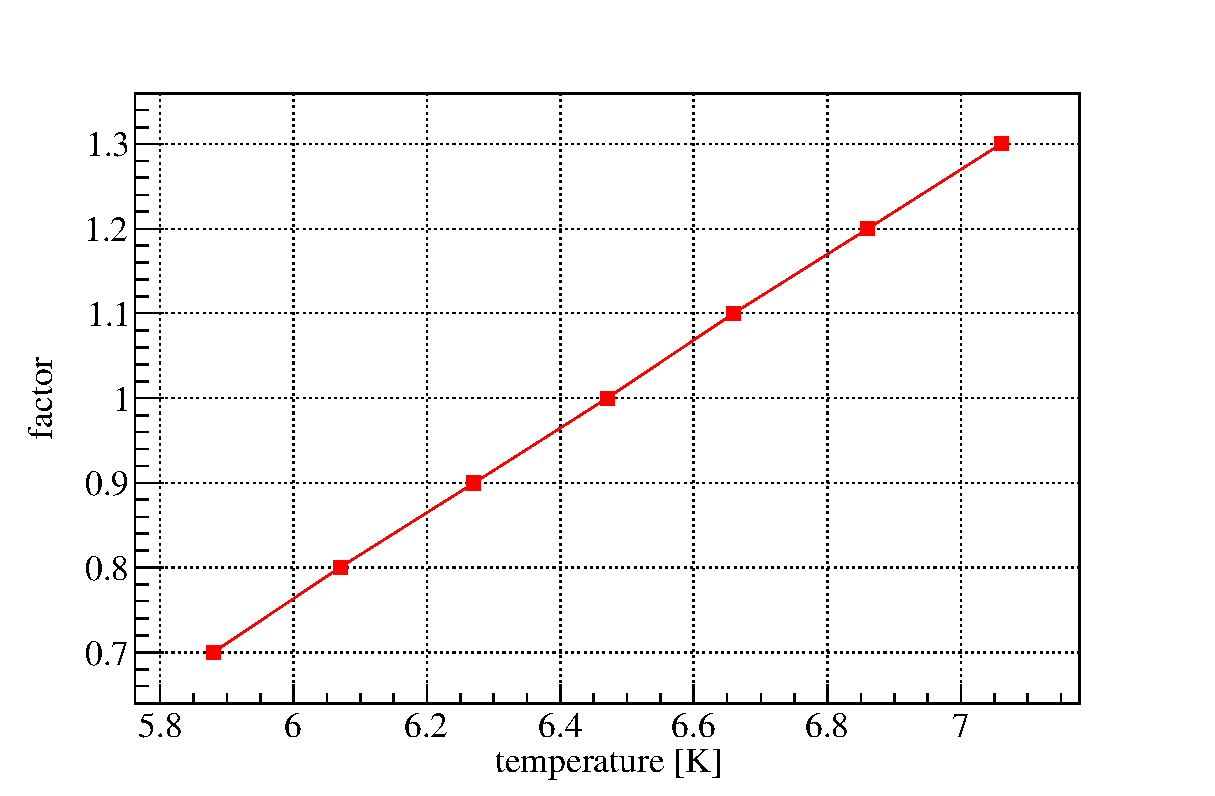
\includegraphics[scale=0.45]{chapter6/fig/factor}
% \caption{\it The temperature peak increases linearly with the energy deposition factor.}
% \label{5factor}
%\end{figure}
%
%\section{New scenario}
%~~~~~~Due to cooling issue of the CS1 coils, the new scenario should be considered if the CS1 cannot be cooled for a long time.
%There are two ways to optimize the CS1 coils to extend the operation time.
%\begin{itemize}
% \setlength{\itemsep}{-5pt}
% \item Using the original design but enlarged the thinckness of aluminium strip.
% \item Seperating the CS1 coils to two parts.
%\end{itemize}
%As shown in figure~\ref{5opti}, the maximum temperature calculated with 90 day operation is able to be reduced by increasing the thickness of aluminium strip.
%If the thickness of aluminium strip can be increased from 1 mm to 2 mm, the peak temperature of 90 day operation is possible to be reduced under current sharing temperature.
%However, increasing the thickness of aluminium strip may make the coil winding become difficult.
%It still needs to discuss in future.
%\begin{figure}[H]
% \centering
% 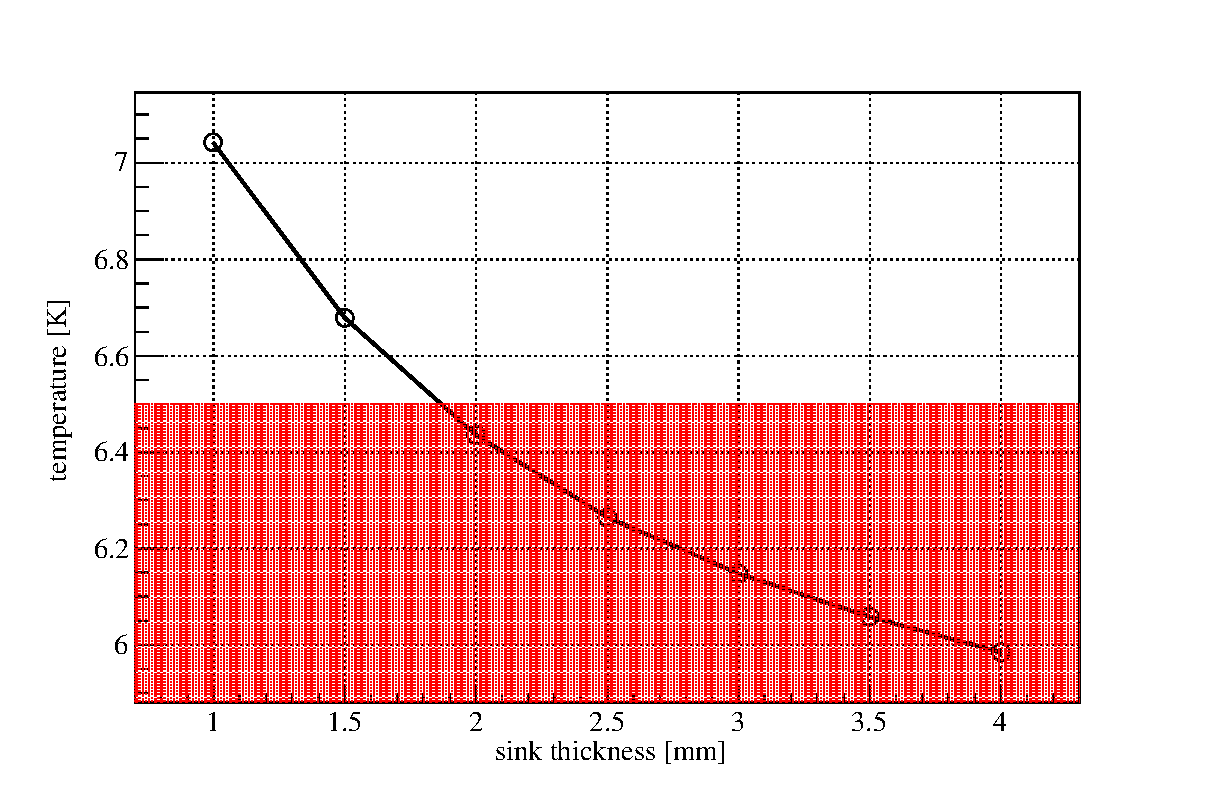
\includegraphics[scale=0.45]{chapter6/fig/Strip}
% \caption{\it The CS1 coils can be optimized by imcreasing the thickness of aluminium strip.}
% \label{5opti}
%\end{figure}
%
%The second scenario is to seperate the CS1 coils to two parts.
%Since the energy deposition peak in the middle of the CS1 coils, seperating the CS1 coils and inserting the aluminium strip in the middle of the CS1 coils, which is shown in figure~\ref{5new}, can help CS1 to be cooled down very well.
%\begin{figure}[H]
% \centering
% 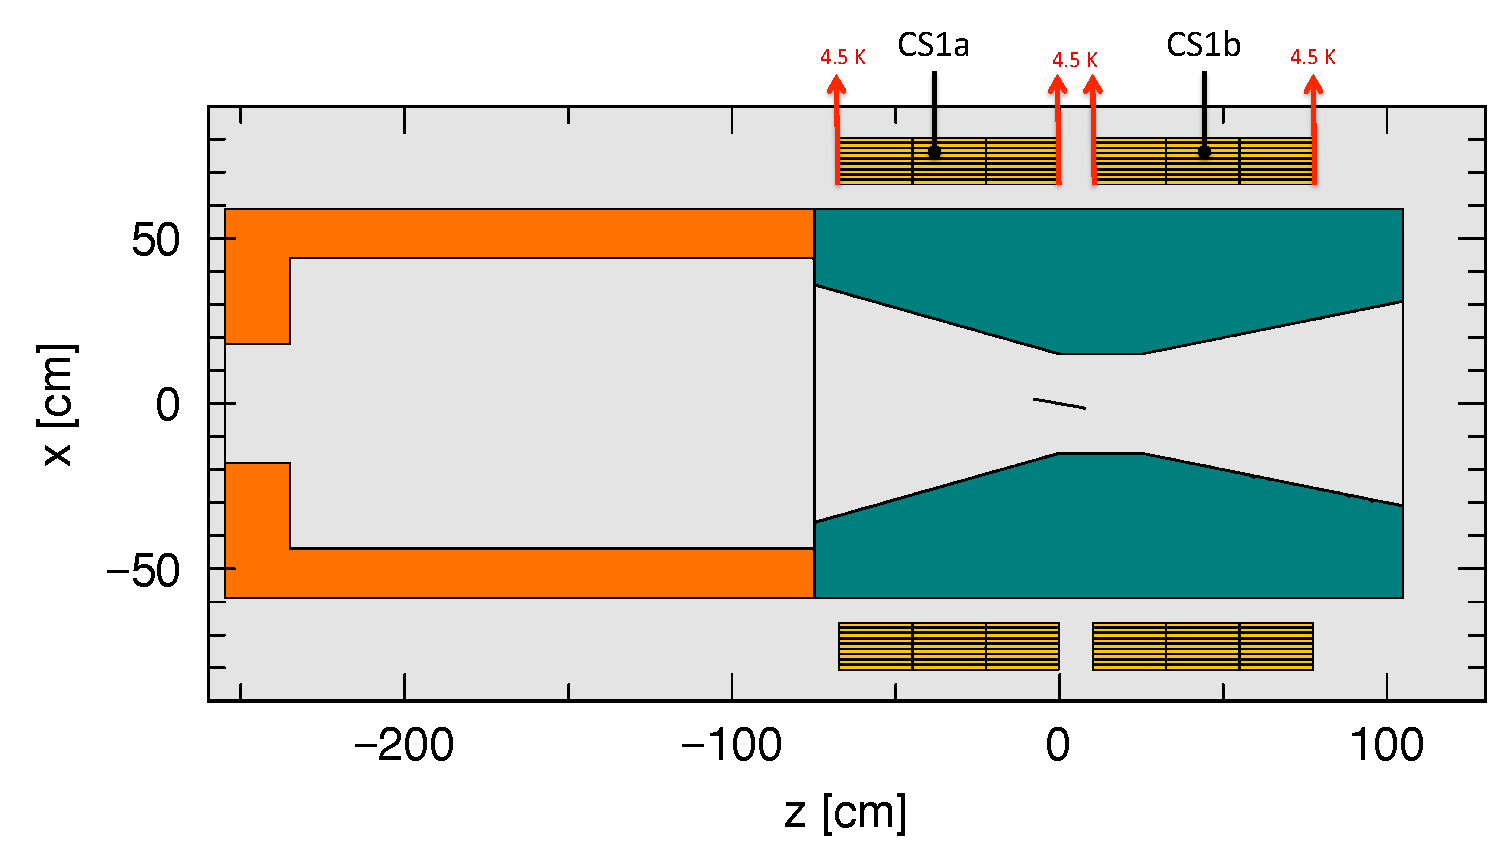
\includegraphics[scale=0.45]{chapter6/fig/CS1new.pdf}
% \caption{\it The scenario of CS1 seperating.}
% \label{5new}
%\end{figure}
%To validate this scenario, the cooling, quench, magnetic field, muon yield and mechanical issue must be estimated.
%

\chapter{Conclusion}
~~~~~~To search for the $\mu^- \rightarrow e^-$ conversion with more precision experimental sensitivity, COMET experiment requires the high intense muon.
8 GeV proton beam with 4.4$\times$10$^{13}$ pps is going to be employed to achieve the high intense muon beam, Thus as the major issue for designing a superconducting magnet system to generate muons, the radiation on COMET superconducting magnet system has been studied in this thesis.

Firstly, radiation on both COMET phase I and phase II are estimated with realistic geometry by using Monte Carlo code.
\begin{itemize}
 \setlength{\itemsep}{-5pt}
 \item COMET superconducting magnets suffer from 1.03$\times$10$^{10}$ n/cm$^2$/sec neutron irradiation ($\textgreater$ 0.1 MeV) for phase-II experiment, which corresponds to 2.49$\times$10$^{21}$ n/m$^2$ neutron fluence totally.
 %\item Over 10$^{21}$ n/m$^2$ neutrons will hit the magnets at peak for 280 day operation in phase-II experiment.
 \item About 3.74 mSv/h residual radiation is still remained after 1-month operation and 10-month cooling for phase-I experiment.
 \item A new radiation shield is designed for both phase-I and phase-II experiment to protect CS and MS superconducting coils from the radiation.
\end{itemize}

Secondly, considering the radiation induced damage on material used in COMET superconducting magnet system, several irradiation tests for GFRPs, quench protection diode, insulation tape and 5N aluminium is carried out.
\begin{itemize}
 \setlength{\itemsep}{-5pt}
 \item The tensile strength of BT is about 375 MPa without irradiation and drops to about 320 MPa after 200 MGy irradiation, which is stronger than G10 and CE
 %\item The tensile strength of G10 and CE without irradiation is lower than BT and BMI's.
 %\item The tensile strength of BT has no big change even with 200 MGy irradiation.
 \item The forward voltage of quench protection diode increases about 0.08 V after total 9.7$\times$10$^{11}$ n/m$^2$ neutron irradiation.
 \item With fitting the cryogenic property of quench protection diode, we estimate its forward voltage will grow up from 0.9 V to about 1.5 V at 210 A and 4.2 K after 10$^{12}$ n/m$^2$ neutron irradiation, and its temperature rises from 4.2 K to 11 K.
 \item Among the several samples of insulation tape, BTGK-C has good mechanical property which has tensile strength of 14 MPa.
 \item The enhanced tensile strength of insulation tape has been observed after 10 MGy irradiation by cobalt source.
 \item According to the neutron irradiation test of 5N aluminium, the RRR of stabilizer drops lower than 100 after 3-month operation.
\end{itemize}

Thirdly, due to the degradation of the stabilizer and aluminium strip which may lead to the issue of cooling and quench, the temperature during the cooling is estimated by solving the three dimensional heat equation.
As for the most dangerous coil in COMET superconducting magnet system, CS1, which is longest one and close to the production target, its temperature margin is estimated to 6.8 K for 30-day operation which exceeds to the current sharing temperature, 6.5 K.
Therefore, to design a superconducting magnet what can operate under the high radiation environment for long time, original design of CS1 solenoid is optimized as follows.
\begin{itemize}
 \setlength{\itemsep}{-5pt}
 \item Shorten the length of aluminium strip from edge of coils to cooling pipe.
 \item Enlarge the length of inner aluminium strip.
 \item Insert the aluminium strip into each layer from two sides.
\end{itemize}
The temperature can be controlled around 5.6 K for 30-day operation with these modification.
As for the quench issue, the maximum temperature of pion capture solenoid is estimated by the worst circumstances.
The quench will lead the temperature to 250 K with 500 V power supply if the RRR of aluminium drops to 100.
The voltage of power supply should be increase to 600 V to secure the temperature after quench.

Therefore, as for nowadays' design for the superconducting magnets of CS1 coils, 30 day operation is fully possible.
However, if the experiment requires for more operation time, the optimization of design should focus on how to cool the CS1 coils efficiently.
